\chapter{Stato dell'arte}

\label{ch:state of the art}

La sicurezza delle password al giorno d'oggi riveste un ruolo significativo nel garantire confidenzialità e integrità dei dati personali degli utenti e delle aziende. 
Solitamente si è più propensi a scegliere password semplici da ricordare, come riferimenti autobiografici, oppure sequenze di caratteri molto comuni (e.g. \texttt{qwerty}, \texttt{123456}).
Per semplificare la memorizzazione, si utilizzano spesso passsword brevi, in media da 9-10 caratteri e composte in gran parte da caratteri minuscoli~\cite{obspasshab}.

Tuttavia questa scelta porta a maggiori probabilità di subire violazioni dei propri account, poiché password semplici sono vulnerabili ad attacchi di forza bruta. Inoltre, tramite tecniche di ingegneria sociale, è possibile individuare il criterio di scelta dell'utente, eventualmente ragionando sui dati disponibili grazie ai data breach.

Nel 2020 sono stati confermati 3950 data breach, dal costo medio di 3,86 milioni di dollari. Il 52\% dei breach è stato causato da attacchi informatici e il numero di giorni medio per individuare un breach è stato di 207 giorni~\cite{ibmcost}.
Il 42\% è causato da attacchi su applicazioni web e il il metodo più comune di attacco (82\%) ha utilizzato credenziali rubate o ottenute tramite attacchi a forza bruta.
Il 58\% dei breach conteneva dati personali~\cite{verizon}.
\begin{figure}[h]
    \centering
    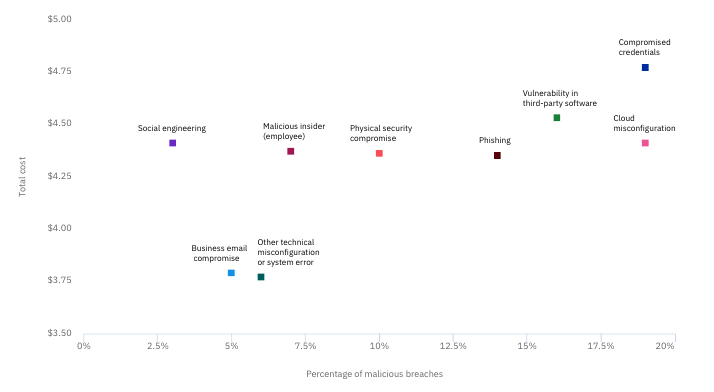
\includegraphics[width=15cm]{./immagini/average_cost_and_frequency_data_breaches.png}
    \label{data breach}
    \caption{Costo medio e frequenza di data breach causati da attacchi informatici, in base alla causa, nel 2020~\cite{ibmcost}}
\end{figure}

Sebbene la maggior parte delle password siano crittografate, è possibile risalire alla forma testuale mediante strumenti come Hashcat\footnote{\url{https://scholar.google.com/scholar?hl=en&as_sdt=0\%2C5&q=hashcat&btnG=}} e John The Ripper.

In seguito alla diffusione delle credenziali, gli utenti decidono di cambiare password e la scelta ricade spesso su varianti usate su altri account.
\section{Scelta di una nuova password}

L'utente medio ha la tendenza a scegliere password semplici~\cite{obspasshab}. Per questo motivo, spesso la nuova password è il risultato di una leggera variazione della vecchia password, o una combinazione di password precedenti~\cite{hypr}.

Un modo per verificare la sicurezza della password è utilizzare strumenti come \href{https://github.com/dropbox/zxcvbn}{zxcvbn}, che riesce a riconoscere:
\begin{itemize}
    \item 30000 password comuni;
    \item nomi e cognomi comuni negli USA;
    \item parole spesso utilizzate in inglese su Wikipedia;
    \item parole spesso utilizzate alla televisione e film statunitensi;
    \item date;
    \item ripetizioni di lettere (\texttt{aaaa});
    \item sequenze alfabetiche (\texttt{abcde});
    \item sequenze di tastiera (\texttt{qwertyuiop});
    \item il codice \texttt{l33t}.    
\end{itemize}

Altri strumenti, come \href{https://password.kaspersky.com/it/}{Kapersky password checker}, controllano anche dati di numerosi data breach raccolti da \href{https://haveibeenpwned.com/}{Have I been Pwned?}.
Questi approcci, tuttavia, non controllano la cronologia delle password di uno specifico utente, ma soltanto la resistenza ad attacchi di forza bruta.

Per questo motivo sono state studiate strategie che tengono conto delle credenziali utilizzate.
Alcune sfruttano un approccio probabilistico, come i \emph{Bloom Filter}, che...*TODO*. Un'altra possibile modalità utilizza \emph{Word Embedding} di password.

\section{Bloom filters}

TODO

\section{Word embedding}
Per capire il contesto delle parole e per poterle rappresentare in base alla sfera semantica e alla sintassi, si ricorre un insieme di tecniche che prevedono il \textit{mapping} delle parole o delle frasi di un dizionario in vettori di numeri reali, note come \emph{Word Embedding}.
Parole simili possiedono una codifica simile.


Per stabilire il valore di ogni \textit{embedding} si allena una rete neurale con specifici parametri e le dimensioni variano tra 8 (per piccoli dataset) a 1024. Maggiore è la dimensione di un embedding, maggiore risulta la quantità di informazioni relativa alle relazioni tra parole~\cite{tensword}.

\subsection{Similarità tra parole}

Per potere stabilire se due parole appartengono alla stessa sfera semantica si utilizza un metodo noto come \emph{cosine similarity}.
\begin{equation}
    similarity = cos(\theta) = \frac{A\cdot{B}}{\|A\|\cdot{\|B\|}}
\end{equation}

Due parole risultano simili quando il valore del coseno è 1, ovvero quando l'angolo tra i due vettori risulta nullo. Si consideri il seguente esempio:

\begin{figure}[h]
    \centering
    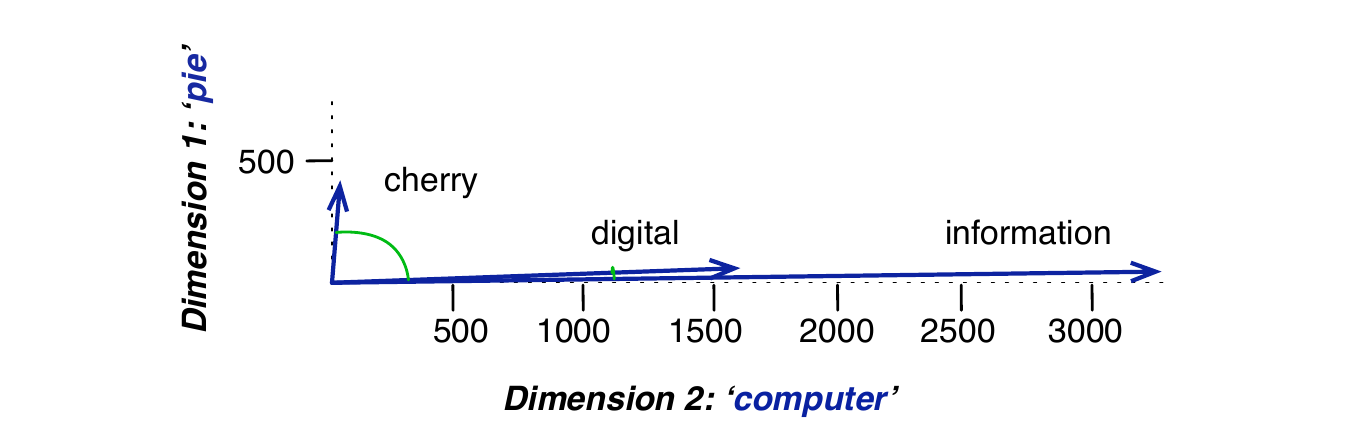
\includegraphics[width=11cm]{./immagini/cosine_similarity_esempio.png}
    \label{cosine}
    \caption{Esempio di calcolo della similarità tra word embedding~\cite{cosine}}
\end{figure}

Nella figura sono mostrati i vettori di 3 parole (\textit{cherry}, \textit{digital} e \textit{information}) in uno spazio bidimensionale definiti dal numero di occorrenze in vicinanza alle parole \textit{computer} e \textit{pie}.
Notare che l'angolo tra \textit{digital} e \textit{information} risulta minore rispetto all'angolo tra \textit{cherry} e \textit{information}.
Quando due vettori risultano più simili tra loro, il valore del coseno risulta maggiore, ma l'angolo risulta minore. Il coseno assume valore massimo 1 quando l'angolo tra i due vettori risulta nullo (0°); il coseno degli altri angoli risulta inferiore a 1~\cite{cosine}.
\subsection{Tipologie di word embedding}

\subsubsection{Word2Vec}

Word2Vec è un insieme di modelli architetturali e di ottimizzazione utilizzati per imparare \emph{word embedding} da un vasto corpus di dati, sfruttando reti neurali.
\\
Un modello allenato con Word2Vec riesce a individuare le parole simili tra loro, in base al contesto, grazie alla \textit{cosine similarity} esaminata precededentemente.

\begin{figure}[h]
    \centering
    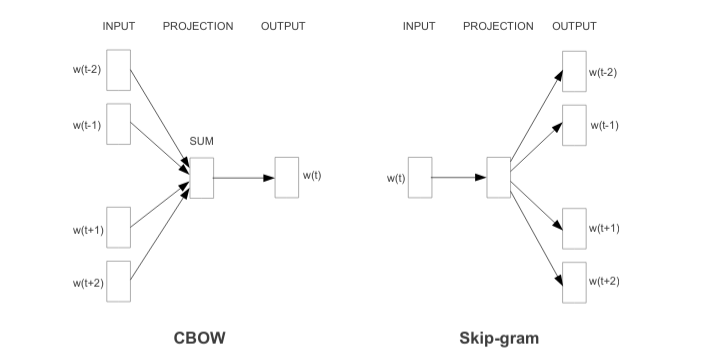
\includegraphics[width=15cm]{./immagini/cbow_vs_skipgram.png}
    \label{cbowskipgram}
    \caption{CBOW vs skip-gram~\cite{mikolov2013efficient}}
\end{figure}
\newpage
Word2Vec utilizza due modelli di architetture:
\begin{itemize}
    \item \emph{CBOW} (continuous bag of words): l'obiettivo del training è combinare le rappresentazioni delle parole limitrofe per prevedere la parola centrale.
    \item \emph{Skip-gram}: simile a CBOW, con la differenza che viene utilizzata la parola centrale per prevedere le parole circostanti relative allo stesso contesto.
\end{itemize}

\emph{CBOW} risulta più veloce ed efficace in caso di dataset di grandi dimensioni, tuttavia, nonostante la maggiore complessità, \emph{Skip-gram} è in grado di trovare parole mai viste, per dataset di minori dimensioni~\cite{mikolov2013efficient}.


\subsubsection{FastText}

FastText è una libreria open-source proposta da Facebook che estende Word2Vec, e consente un apprendimento efficiente di rappresentazioni di parole e di classificazioni di frasi.
Anziché allenare un modello fornendo ogni singola parola di un dataset, FastText prevede l'apprendimento tramite \textit{n-gram} di ciascuna parola.
Un esempio per capire cosa siano effettivamente gli n-gram è il seguente:

\begin{center}
    $ciao = \{\{c, i, a, o\},\{ci, ia, ao\}, \{cia, iao\}, \{ciao\}\}$
\end{center}

In questo esempio, con $n\_mingram = 1$ e $n\_maxgram = 4$, $ciao$ viene espresso come l'insieme di tutte le sottostringhe di lunghezza minima pari a 1, e lunghezza massima pari a 4.


FastText consente di ottenere, con più probabilità rispetto a Word2Vec, parole \emph{out-of-dictionary}, ovvero parole sconosciute al modello in fase di training.

TODO:

\begin{enumerate}
    \item Rifare figura 1.1 su GIMP
\end{enumerate}
